%%
%% licence       kaneton licence
%%
%% project       kaneton
%%
%% file          /home/buckman/kaneton/view/book/assignments/2007/k4/k4.tex
%%
%% created	 pidancet julian	[tue may29 16:34:56 2006]
%% updated	 pidancet julian	[tue may29 16:34:56 2006]
%%

%
% k2
%

\chapter{K4: IPC Management}
\begin{tabular}{p{7cm}l}
Duration: & 2 weeks \\
Directory name: & kaneton/ \\
In charge: & Julian Pidancet, Matthieu Bucchianeri \& Renaud Voltz\\
Mailing-list: & kaneton-students@googlegroups.com \\
Languages: & C, assembly \\
Students per group: & 2 (same groups as for K3) \\
\end{tabular}

\section{Abstract}

K4 implements the last part of our microkernel: IPC (Inter-process
Communication). In a microkernel, on the contrary to a monolithic kernel,
every kernel services are running independently from the core, in separate
userspace tasks. In order to communicate, they need to interact: sending,
receiving messages, and synchronizing each others. The IPC model chosen for
kaneton is {\bf message passing}.

Concerned parts are:

\begin{enumerate}
  \item
    {\bf The message manager, messaging primitives (1)} \\
    Inter-process messaging primitives. Send and receive functions,
    synchronous and asynchronous.
  \item
    {\bf The message manager, IA-32 Syscall Handlers (2)}\\
    Handling kernel-side soft-interrupts (syscalls to the messaging
    primitives).
  \item
    {\bf Task side, IA-32 Syscall Triggers (3)}\\
    Userland syscall functions (sends soft interrupts to the kernel to
    send a message from userland).
\end{enumerate}

\begin{center}
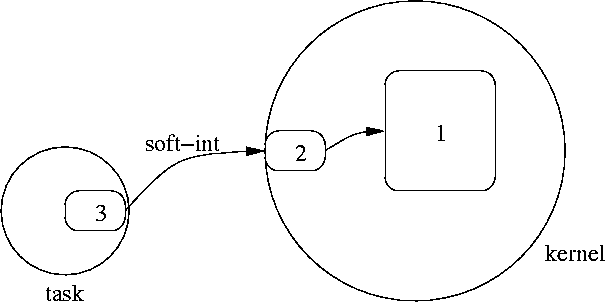
\includegraphics[width=0.5\linewidth]{figures/message.png}
\end{center}

\newpage

\section{message manager, \textbf{messaging primitives}}

\begin{itemize}
  \item {\bf Assignments (architecture-independent)}

    Implement the messaging primitives to send and receive messages in both
    asynchronous and synchronous modes. These primitives will be invoked by
    syscalls, to permit running tasks sending and receiving messages to and
    from userspace (see the 2 next sections).

  \item {\bf Interface}

    \function{message\_async\_send}{(i\_task \argument{sender},
      i\_node \argument{dest},
      t\_tag \argument{tag},
      t\_vaddr \argument{data},
      t\_vsize \argument{size})}
	 {
	   \item \argument{dest}

	     contains the {\bf taskid} and the {\bf machineid} to which the
	     message must be sent asynchronously (\textbf{machineid} is ignored).

	   \item \argument{sender}

	     Identifier of the sending task. Set by the kernel syscall
	     handlers with \textbf{task\_current()}.

	   \item \argument{tag}

	     Ignored. It will be used in the future to apply selection on
	     the queued messages in a task's message box.

	   \item \argument{data}

	     Virtual address of the buffer to be transmitted. Be carreful,
	     this address is not always mapped in the kernel address
	     space. \argument{data} address space is stored in the
	     \argument{sender}'s \textbf{o\_task}.

	   \item \argument{size}

	     Size of the message in the \argument{data} buffer.
	 }
	 
\function{message\_async\_recv}{(i\_task \argument{receiver},
				 t\_tag \argument{tag},
				 t\_vaddr \argument{buff},
				 t\_vsize \argument{buffsz},
				 i\_node* \argument{sender},
				 t\_vsize* \argument{msgsz})}
	 {
	 \item This primitive receives an asynchronous message. It returns
	   an error if no message is pending for the \argument{receiver}
	   task.
	     
	 \item \argument{sender}

	   Identifier of the receiving task. Set by
	   the kernel syscall handlers with \textbf{task\_current()}.

	 \item \argument{tag}

	   Ignored. It will be used in the future to
	   apply selection on the queued messages in a task's message box.

	 \item \argument{buff}

	   Virtual address of the receiving
	   buffer. Be carreful, this address is not always mapped in the
	   kernel address space. \argument{buff} address space is stored in
	   the \argument{sender}'s \textbf{o\_task}.

	 \item \argument{maxsz}

	   Size of the receiving buffer, used to avoid buffer overflows.

	 \item \argument{sender} and \argument{msgsz}
	   
	   Pointers used to
	   get back the sender and the size of the received message. Be carefull,
	   these pointers are not refering to the calling task's address space.
	   The return values have to be passed by registers while returning
	   from the syscall.
	 }

\function{message\_sync\_send}{(i\_task \argument{sender},
				i\_node \argument{dest},
				t\_tag \argument{tag},
				t\_vaddr \argument{data},
				t\_vsize \argument{size})}
	 {
	   \item \argument{send}, \argument{dest}, \argument{tag},
	     \argument{data}, \argument{size}

	     See \textbf{message\_async\_send()} for details.
	 }

\function{message\_sync\_recv}{(i\_task \argument{receiver},
				t\_tag \argument{tag},
				t\_vaddr \argument{data},
				t\_vsize \argument{maxsz},
				t\_state \argument{blocking},
				i\_node* \argument{sender},
				t\_vsize* \argument{msgsz})}
	 {
	   \item \argument{blocking}

	     Sets the behaviour of the function if no symetric
	     \textbf{message\_sync\_send()} to task \argument{receiver}
	     happened before. if \argument{blocking} is clear, the function
	     immediatly returns an error. Otherwise, the task
	     \argument{receiver} is blocked until another task tries to
	     synchronize with it.

	   \item \argument{receiver}, \argument{tag}, \argument{data},
	     \argument{sender}, \argument{msgsz}

	     See \textbf{message\_async\_recv()} for details.
	 }


  \item {\bf {Files}}

    \begin{tabular}{| l | l |}
      \hline
      machine-independent & {\em kaneton/core/message/message.c}\\
      &  {\em kaneton/include/core/message.h}\\\hline
    \end{tabular}
\end{itemize}

\section{message manager, \textbf{IA-32 syscalls handlers}}
\begin{itemize}
  \item {\bf Overview}

    This part of the code is used to hook software interrupts to your
    handlers. Handlers must:

    \begin{enumerate}
      \item fetch the passed arguments from the interrupted context
      \item call the right function of the message manager
      \item write its result back into the interrupted context.
    \end{enumerate}

  \item {\bf Assignments (architecture-dependent)}

    Implement the kernel-side of the syscalls that will invoke the messaging
    functions.

    No special model is imposed. You can either dispatch your syscalls by hand
    (using a single interrupt gate and passing an identifer as an argument),
    or let the microprocessor do it for you (using one specific gate for each
    syscall).

  \item {\bf {Files}}

    \begin{tabular}{| l | l |}
      \hline
      machine-dependent & {\em kaneton/core/arch/ibm-pc.ia32-virtual/message.c}\\
      & {\em kaneton/include/arch/ibm-pc.ia32-virtual/core/message.h}\\\hline
    \end{tabular}

\end{itemize}

\newpage

\section{Task side, \textbf{IA-32 syscall triggers}}
\begin{itemize}
  \item {\bf Overview}

    This portion of code is used by user (and kernel) tasks. IRL,
    it would be located in the libc (like in UNIX systems, the
    \emph{read} function that does the read syscall is located in the
    libc), but as the kernel code is always mapped to make the debug
    and testing easier, it will be put into this code.

    Each function must:

    \begin{enumerate}
      \item Put the incoming arguments in registers
      \item Trigger the right software interrupt
      \item Get back the results from the registers to the outgoing arguments
    \end{enumerate}

  \item {\bf Assignments (architecture-dependent)}

    Implement the 4 syscalls so the userland tasks can call the
    message manager into the kernel.

    XXX

  \item {\bf Interface}

    \function{syscall\_async\_send}{(i\_node \argument{dest},
				 t\_tag \argument{tag},
				 void* \argument{data},
				 t\_size \argument{size})}
	     {}
	 \function{syscall\_async\_recv}{(t\_tag \argument{tag},
				 void* \argument{buff},
				 t\_size \argument{maxsz},
				 i\_node* \argument{sender},
				 t\_size* \argument{msgsz})}
		  {}
	 \function{syscall\_sync\_send}{(i\_node \argument{dest},
				t\_tag \argument{tag},
				void* \argument{data},
				t\_size \argument{size})}
		  {}
	 \function{syscall\_sync\_recv}{(t\_tag \argument{tag},
				void* \argument{buff},
				t\_size \argument{maxsz},
				t\_state \argument{blocking},
				i\_node* \argument{sender},
				t\_size* \argument{msgsz})}
		  {}

		  See above sections for more information about functions
		  parameters

  \item {\bf {Files}}

    \begin{tabular}{| l | l |}
      \hline
      machine-dependent & {\em kaneton/core/arch/ibm-pc.ia32-virtual/message.c}\\
      & {\em kaneton/include/arch/ibm-pc.ia32-virtual/core/message.h}\\\hline
    \end{tabular}

\end{itemize}

%
% appendix
%

\newpage

\section{Appendix}

\textbf{Example of messaging syscall use: let us consider this amayzing scenario:}
\begin{itemize}
  \item task\_1 sends ``ping'' to task\_2
  \item task\_2 answers ``pong'' to task\_1
\end{itemize}


\begin{enumerate}
  \item Using synchronous send and receive, task\_1 and task\_2 first
    synchronize together (because both \textbf{sync\_send} and
    \textbf{sync\_recv} are blocking), the string ``ping'' is then copied
    directly from task\_1 address space to task\_2 address space.

  \item	Then task\_1 enters in a polling loop, waiting for an answer, because
    task\_2 answers in asynchronous mode. The string ``pong'' is copied into
    task\_1 address space in two stepss: message is queued into the kernel
    memory between the two calls.
\end{enumerate}

\begin{itemize}
  \item Task 1
\begin{verbatim}
void             tsk1_main()
{
  char          *to_send = "ping";
  i_node        dest;

  char		recv[64];
  i_node	from;
  t_size	recv_sz = 0;

  dest.task = 2;

  /* Synchronize to task 2 and send "ping" */
  syscall_sync_send(dest, 0, to_send, 5);

  /* Polling to receive a message */
  while (syscall_async_recv(0, recv, 64, &from, &recv_sz) != ERROR_NONE
         && from != 2)
    ;
}
\end{verbatim}

  \item Task 2
\begin{verbatim}
void             tsk2_main()
{
  char          *to_send = "pong";
  i_node        from;
  char		recv[64];
  t_size	recv_sz = 0;

  /* Synchronize, and receive a message */
  syscall_sync_recv(0, recv, 64, 1, &from, &recv_sz);

  /* Answer asynchronously */
  syscall_async_send(from, 0, to_send, 5);
}
\end{verbatim}

\end{itemize}
